\newpage
\section{Appendix}
\label{sec:Appendix}

\subsection*{Video-Super-Resolution using Optical Flow Reconstruction}
One approach that was tried in order to apply \ac{TAD} on \ac{VSR} was to find a
low-dimensional representation that is optimal to reconstruct the optical flow.
\myfigref{fig:architecture_video_flow} indicates the design for this
approach, which was trained using the UCL optical flow dataset (\cite{ADAEMFOF})
and the OpenCV Farneback dense optical flow function (since easily available
for a conceptual test).
Unfortunately, the approach did not converge to useful representation. Since
other approaches could successfully solve the \ac{VSR} task this approach was
discarded.

\begin{figure}[!ht]
	\centering
	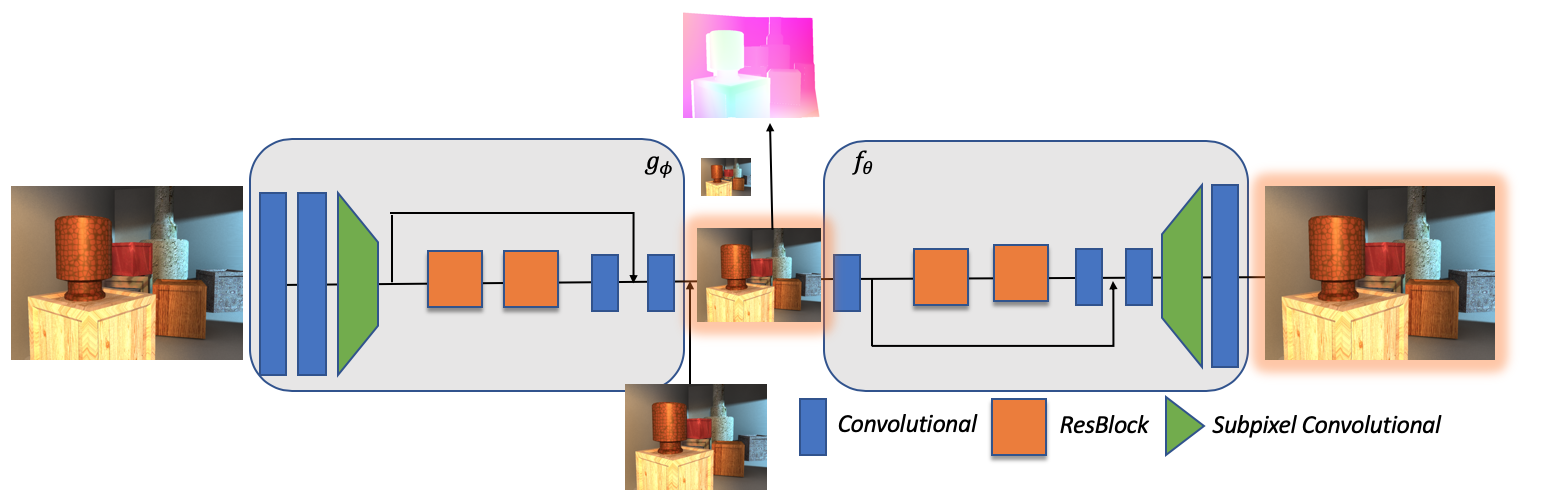
\includegraphics[width=14cm]{figures/architecture_video_flow}
	\caption{Design for \ac{TAD} video super-resolution task (example network
  architecture) for optical flow reconstruction. }
  \label{fig:architecture_video_flow}
\end{figure}

\begin{figure}[!ht]
	\centering
	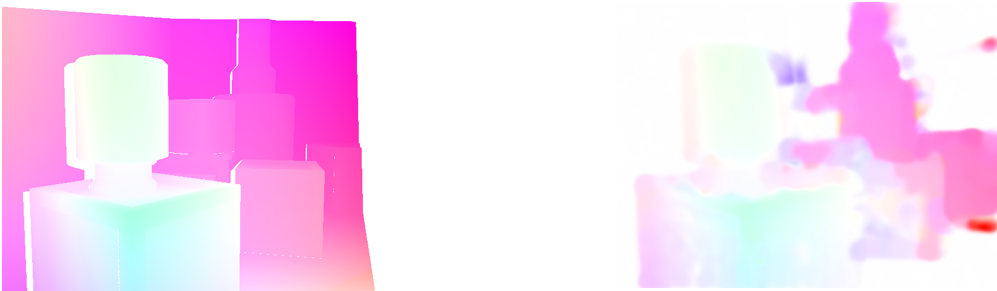
\includegraphics[width=10cm]{figures/flow}
	\caption{Optical flow reconstruction: Groundtruth (left) and reconstructed
  image (right).}
  \label{fig:flow}
\end{figure}

\subsection*{SOFVSR model selection and working principle}
Wang et al. \cite{LFVSRTHROFE} (SOFVSR) implemented an end-to-end trainable
approach to predict both, the \ac{HR} frame as well as the HR optical flow.
Therefore, first the HR optical flow is inferred in a coarse-to-fine manner,
then motion compensation is performed according to the HR optical flows and
finally, the compensated LR inputs are fed to a super-resolution network to
generate the HR frame estimate (comp. \myfigref{fig:sofvsr}).

\begin{figure}[!ht]
	\centering
	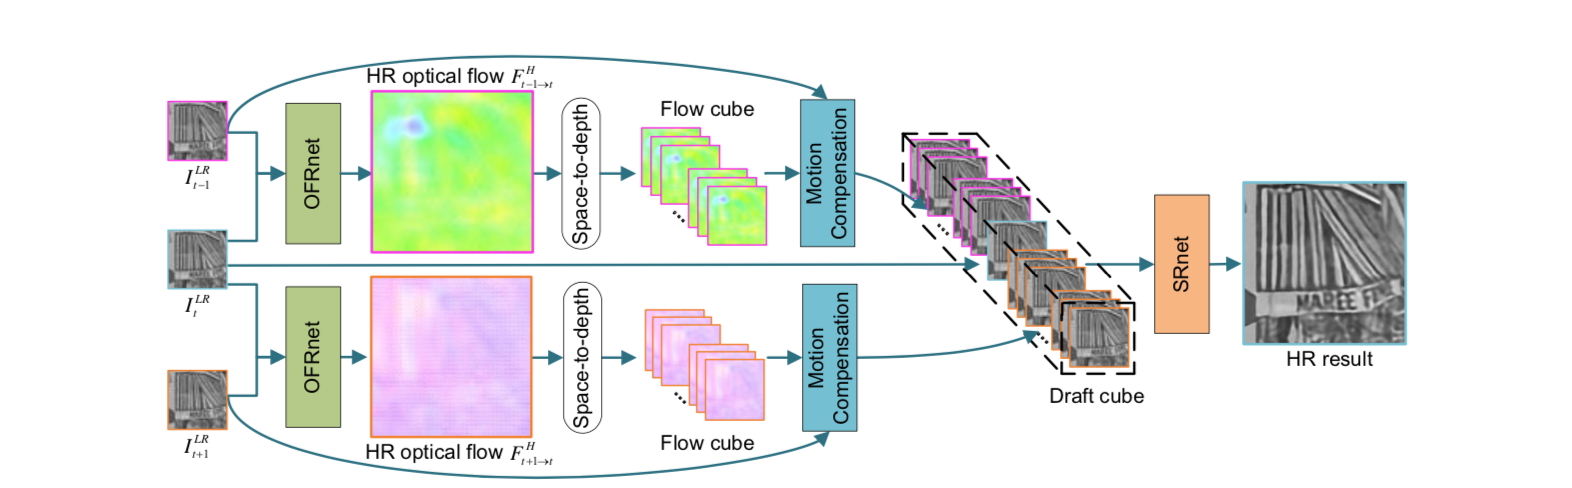
\includegraphics[width=14cm]{figures/sofvsr}
	\caption{Overview of SOFVSR pipeline \cite{LFVSRTHROFE}.}
  \label{fig:sofvsr}
\end{figure}

The SOFVSR model was selected based on a combination of criteria such as the
stated reconstruction performance (PSNR) and runtime, the closeness to
state-of-the-art and the availability of a PyTorch open-source implementation.

\begin{figure}[!ht]
	\centering
	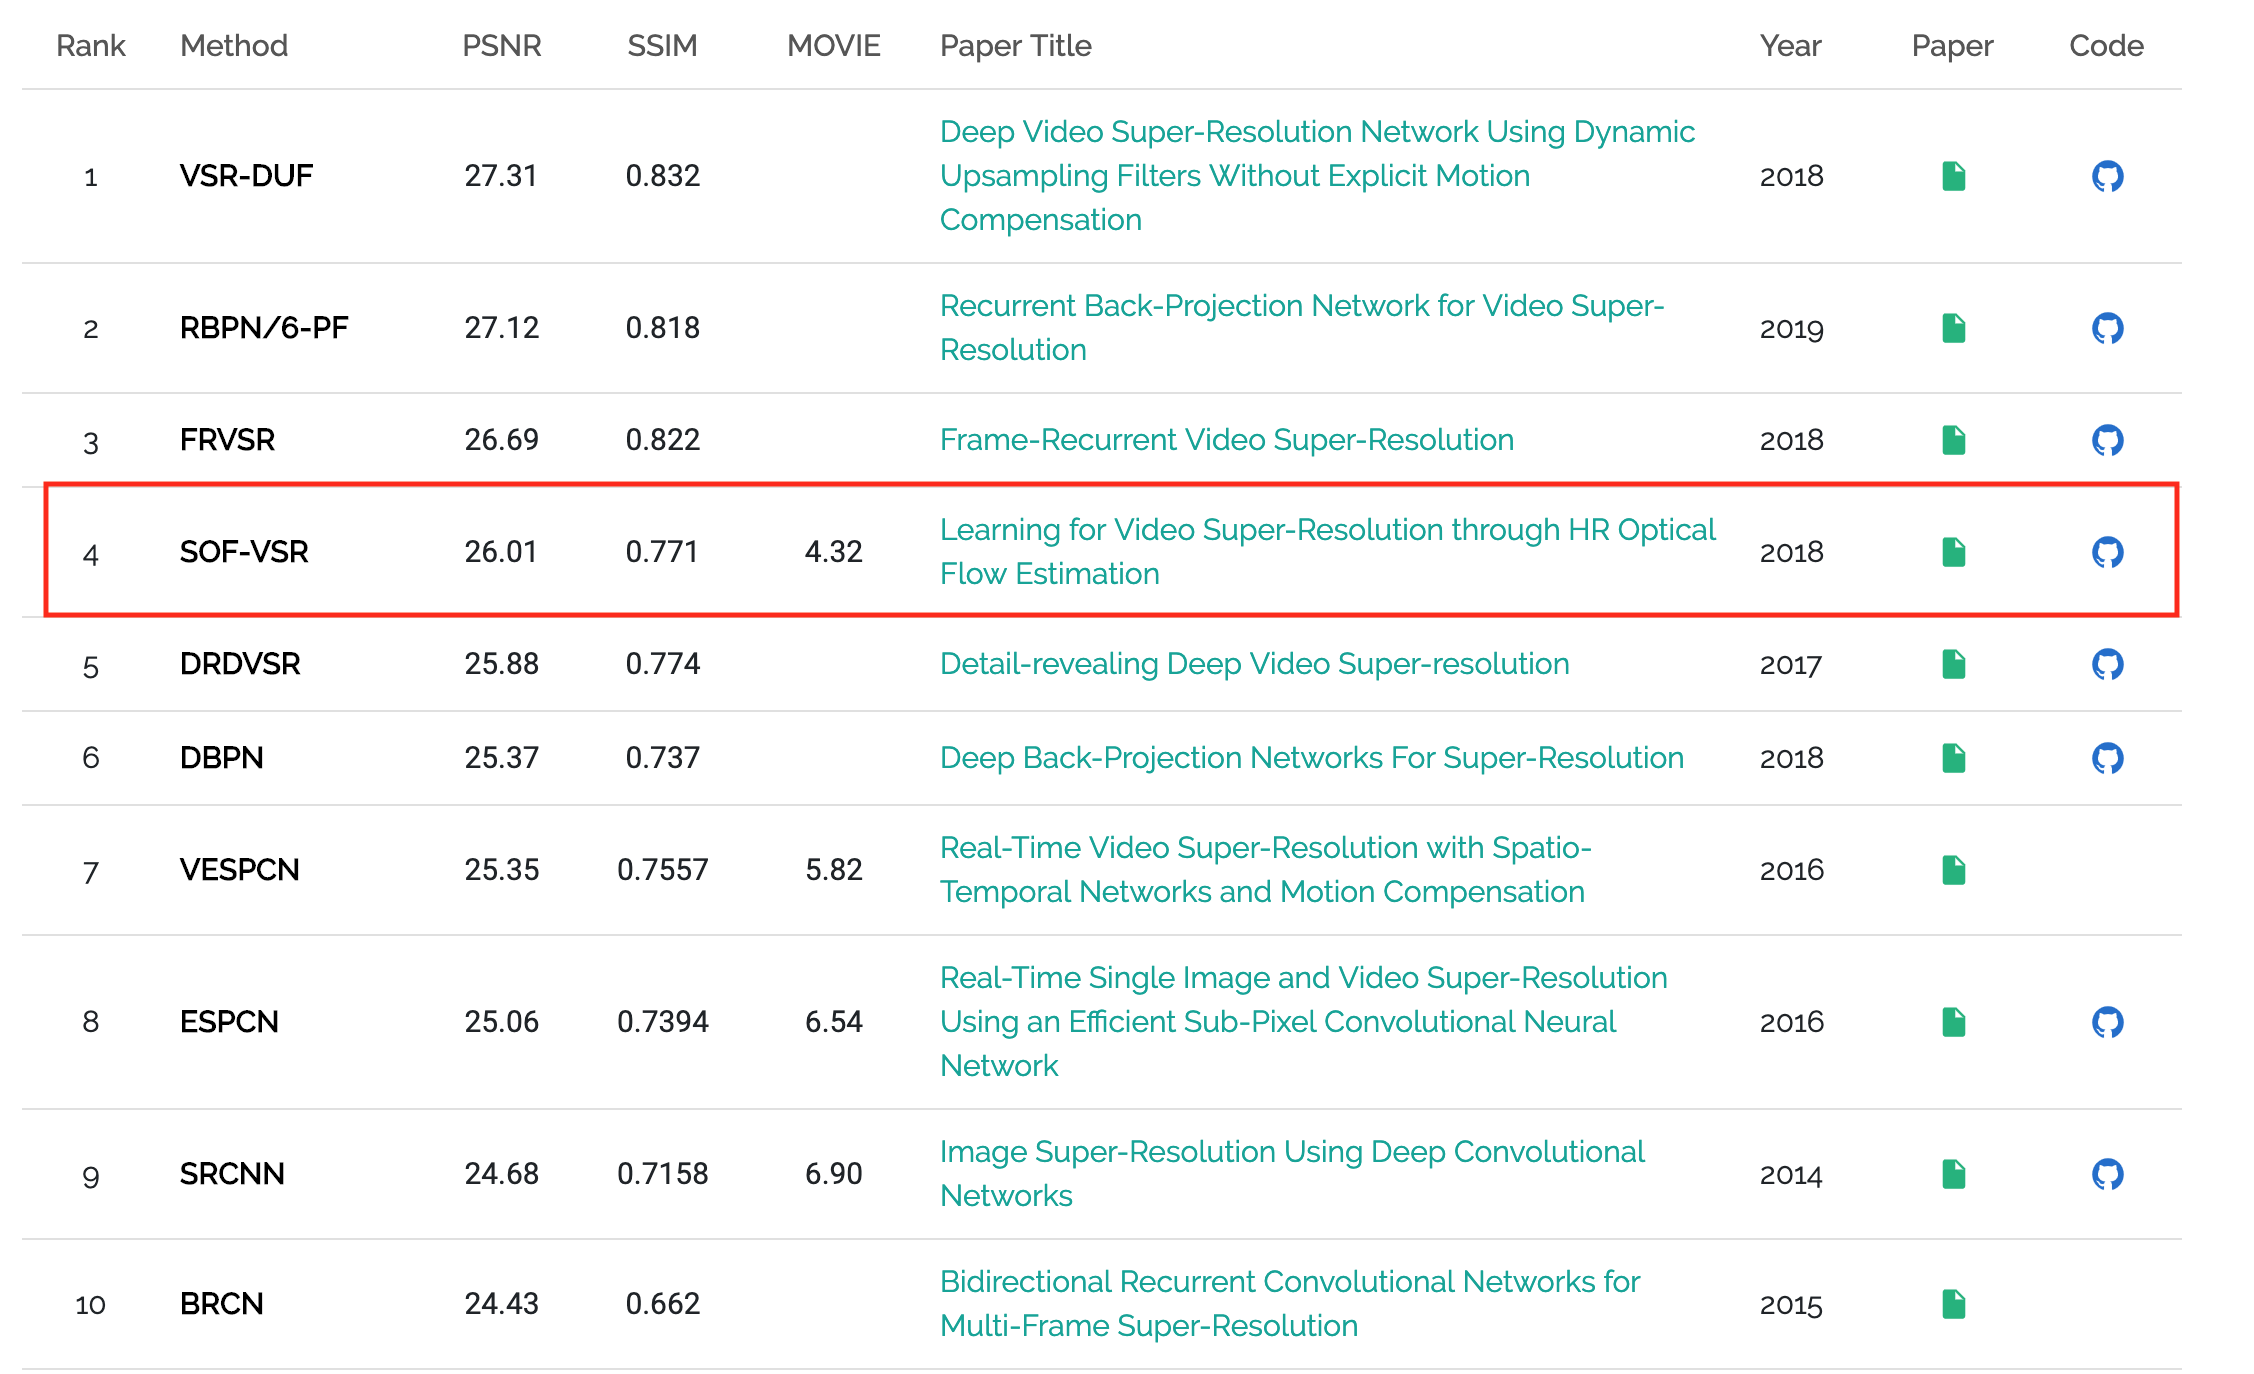
\includegraphics[width=14cm]{figures/sofvsr_selection}
	\caption{Comparison of several \ac{VSR} methods according to PapersWithCode.}
  \label{fig:sofvsr_selection}
\end{figure}

\subsection*{List of Experiments}

\begin{figure}[!ht]
	\centering
	
\includegraphics[width=14cm]{figures/cvl}
	\caption{List of important (non-complete) experiments.}
  \label{fig:experiments}
\end{figure}
